\documentclass{article}
\usepackage{graphicx}
\usepackage{geometry}
\usepackage{float}
\usepackage{fancyhdr}
\usepackage{graphicx}



% Set up page layout
\geometry{a4paper, margin=1in}

% Set up the header
\pagestyle{fancy}
\fancyhf{}
\fancyhead[C]{CMEE Bootcamp Assignment: Sebastian Dohne - 01776389} % Centered header text
\renewcommand{\headrulewidth}{0pt} % Add a horizontal line under the header


\begin{document}

% Centered main section title
\begin{center}
    \section*{Is Florida Getting Warmer?}
\end{center}

% Subsection title
\subsection*{Background and Hypothesis}

The following describes a permutation analysis that was conducted on a dataset containing mean yearly temperature data and their respective years (ranging from 1900-2000) from Key West, Florida to answer the following questions:

\begin{itemize}
    \item Is there a positive correlation between year and temperature? 
    \item If so, is this correlation statistically significant? 
\end{itemize}

\subsection*{Statistical Analyses and results}
 In R version (version 4.3.3, 2024-02-29), a simple Pearson correlation coefficient was calculated using the cor() function between mean yearly temperature and years. This resulted in a moderate positive correlation coefficient of 0.533. To calculate an approximate asymptotic p-value, the temperature data was shuffled, retested, and recorded 10000 times. Then a function was written to calculate the fraction of results that were greater than the initial result, which was interpreted as a p-value. The P-value was found to be 0 indicating a statistically significant correlation between year and temperature result. A linear regression was also fitted between temperature and year with a y intercept of 7.5516 when year is 0 and a slope of 0.0071 increase in temperature year on year.  

\section*{Figure}
\centering
\vspace{2em}

\centering
\begin{figure}[H]
    \centering
    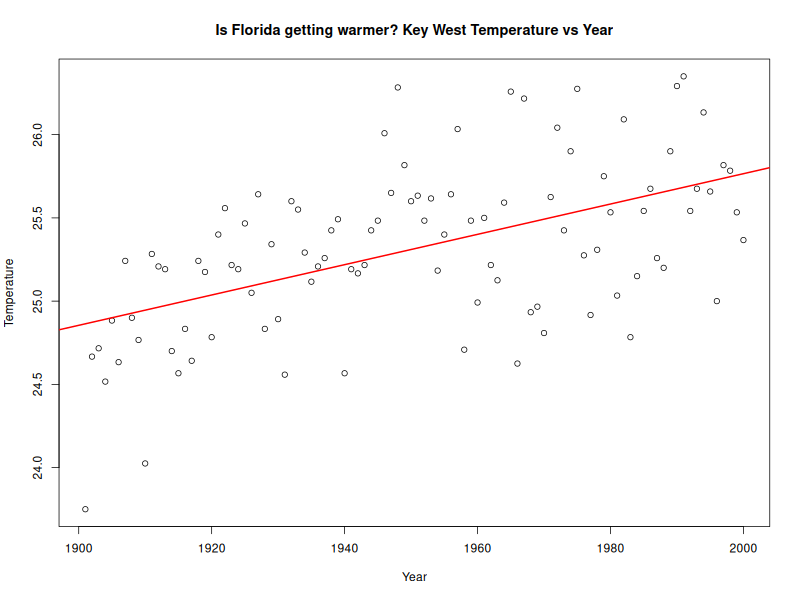
\includegraphics[width=0.9\linewidth]{../data/KeyWest_Temperature_vs_Year.png}
    \vspace{2em}
    \caption[Key West Temperature vs Year]{This figure shows the relationship between year and temperature in Key West, Florida. The red line represents the fitted linear regression model with an intercept of 7.5516 when year is 0 and a slope of 0.0071}
    \label{fig:label2}
\end{figure}

\end{document}
